\documentclass[border=10pt]{standalone}

\usepackage{tikz}
\usepackage{tikzsymbols}
\usetikzlibrary{calc,patterns,shapes.geometric}

\def\centerarc[#1](#2)(#3:#4:#5){\draw[#1] ($(#2)+({#5*cos(#3)},{#5*sin(#3)})$) arc (#3:#4:#5);}

\begin{document}
	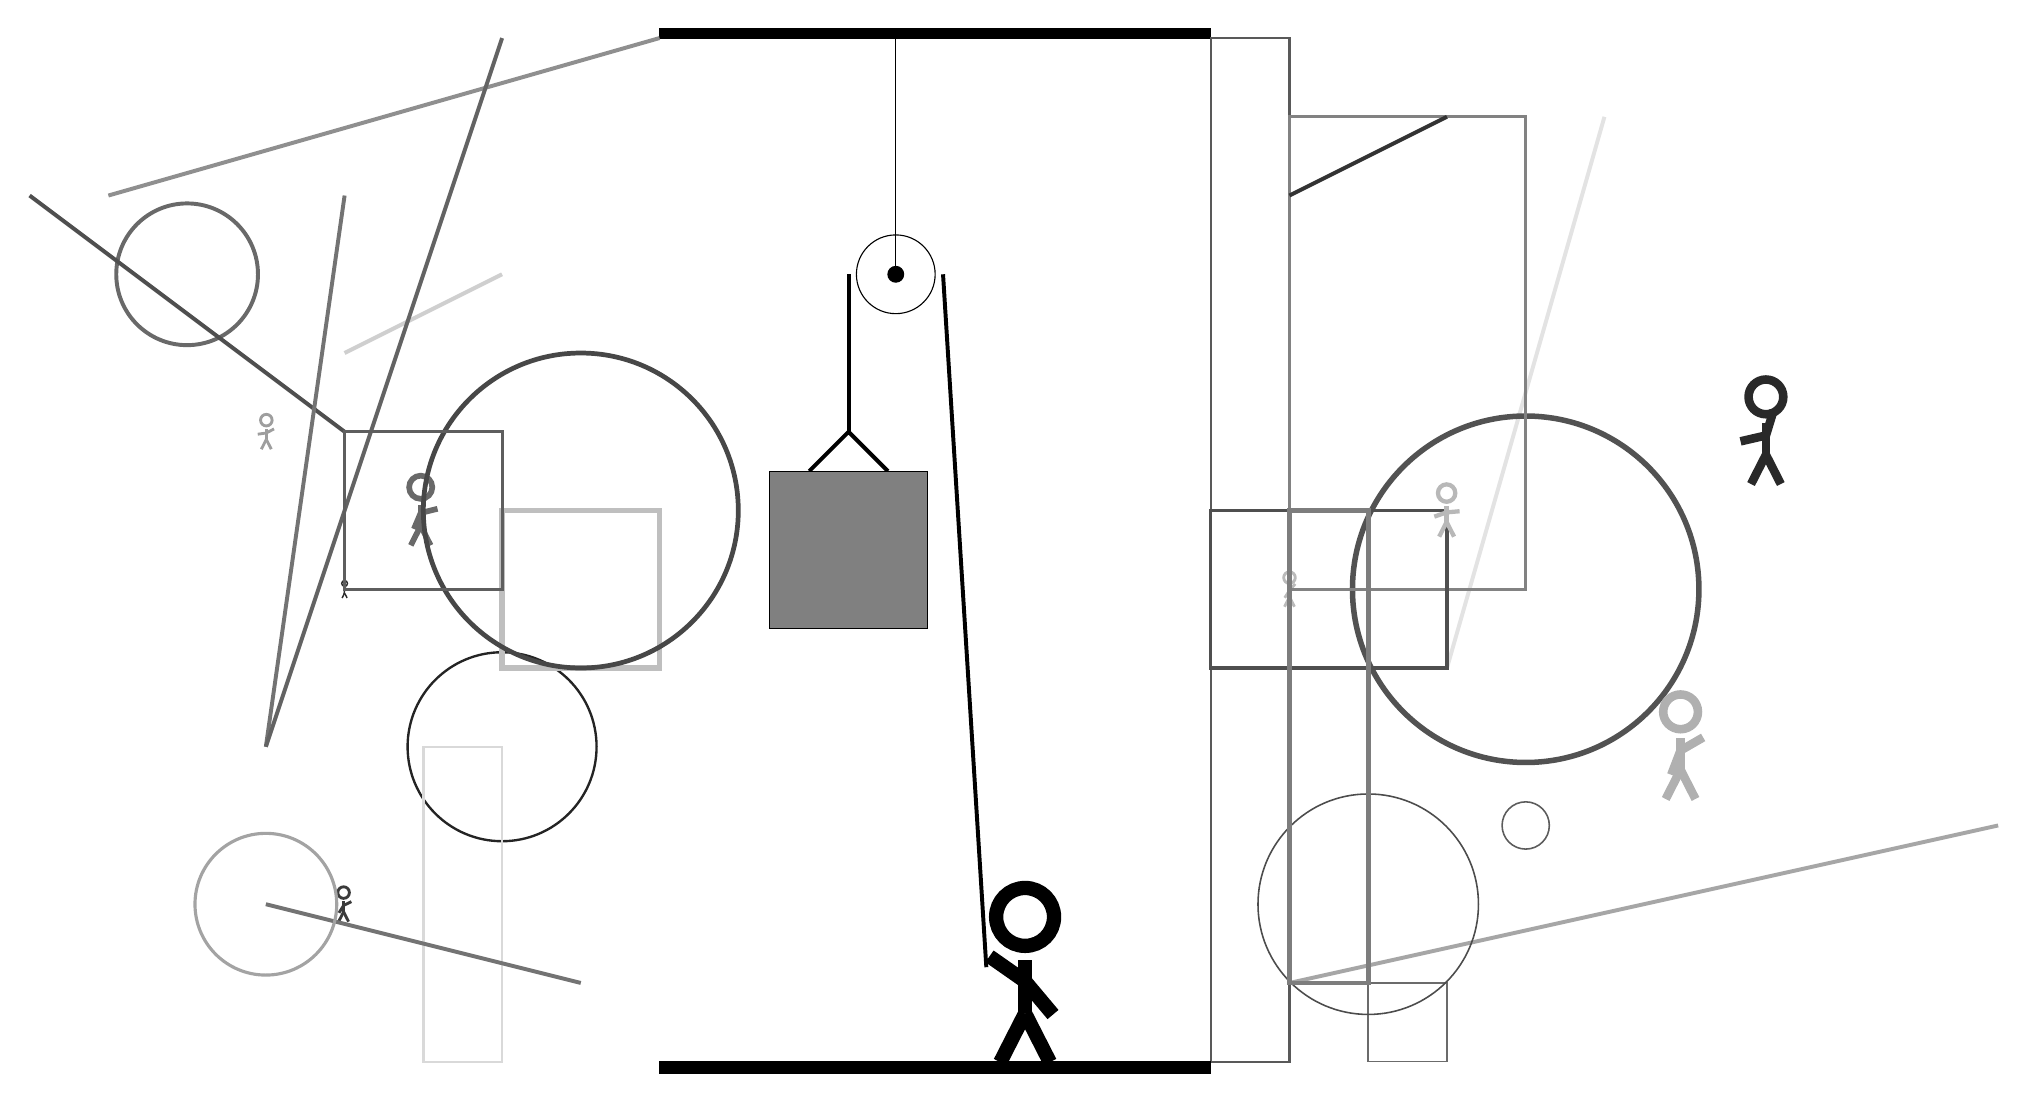
\begin{tikzpicture}
		%%%%% START %%%%%
		
		\draw[fill=black] (-2, 10) rectangle (5, 10.125);
		
		\draw (1, 7) circle (0.5);
		\draw[fill=black] (1, 7) circle (0.1);
		\draw (1, 10) -- (1, 7);
		
		\draw[line width=0.5mm] (-0.1, 4.5) -- (0.4, 5.0) -- (0.9, 4.5);
		\draw[fill=black!50] (-0.6, 4.5) rectangle (1.4, 2.5);
		
		\draw[line width=0.5mm, color=black!19](-4, 7) -- (-6, 6);
		
		\draw[line width=0.5mm, color=black!11](10, 9) -- (8, 2);
		\draw [line width=0.5mm, color=black!59](-8, 7) circle (0.9);
		\node[line width=0.5mm, color=black!83] at (-6, 3) {\Strichmaxerl[1][83][74]};
		\draw [line width=0.3mm, color=black!86](-4, 1) circle (1.2);
		
		\draw [line width=0.7mm, color=black!68](9, 3) circle (2.2);
		\draw[line width=0.5mm, color=black!44](-2, 10) -- (-9, 8);
		
		\draw[line width=0.5mm, color=black!35](6, -2) -- (15, 0);
		\node[line width=0.6mm, color=black!84] at (12, 5) {\Strichmaxerl[6][13][73]};
		
		\node[line width=0.5mm, color=black!31] at (11, 1) {\Strichmaxerl[6][69][30]};
		
		\draw [line width=0.2mm, color=black!64](9, 0) circle (0.3);
		
		\draw[line width=0.3mm, color=black!65] (5, -3) rectangle (6, 10);
		\draw[line width=0.3mm, color=black!15] (-4, -3) rectangle (-5, 1);
		
		\draw[line width=0.5mm, color=black!69](-6, 5) -- (-10, 8);
		\node[line width=0.3mm, color=black!27] at (6, 3) {\Strichmaxerl[2][57][49]};
		\draw[line width=0.2mm, color=black!58] (7, -3) rectangle (8, -2);
		
		\draw[line width=0.5mm, color=black!55](-7, 1) -- (-6, 8);
		\draw[line width=0.4mm, color=black!49] (6, 9) rectangle (9, 3);
		\draw[line width=0.5mm, color=black!80](8, 9) -- (6, 8);
		
		\node[line width=0.4mm, color=black!77] at (-6, -1) {\Strichmaxerl[2][58][26]};
		\draw[line width=0.5mm, color=black!61](-4, 10) -- (-7, 1);
		\draw[line width=0.5mm, color=black!55](-3, -2) -- (-7, -1);
		
		\draw [line width=0.2mm, color=black!70](7, -1) circle (1.4);
		\node[line width=0.3mm, color=black!59] at (-5, 4) {\Strichmaxerl[4][67][14]};
		\draw[line width=0.4mm, color=black!69] (5, 2) rectangle (8, 4);
		\draw[line width=0.7mm, color=black!25] (-4, 2) rectangle (-2, 4);
		\node[line width=0.4mm, color=black!28] at (8, 4) {\Strichmaxerl[3][19][5]};
		\draw [line width=0.6mm, color=black!72](-3, 4) circle (2.0);
		\draw[line width=0.6mm, color=black!51] (7, 4) rectangle (6, -2);
		\node[line width=0.7mm, color=black!38] at (-7, 5) {\Strichmaxerl[2][8][28]};
		\draw[line width=0.4mm, color=black!63] (-4, 3) rectangle (-6, 5);
		
		\draw [line width=0.4mm, color=black!36](-7, -1) circle (0.9);
		
		\draw[line width=0.5mm] (0.4, 7) -- (0.4, 5.0);
		\centerarc[line width=0.5mm](1, 7)(0:180:0.6);
		\draw[line width=0.5mm](1.6, 7) -- (2.15, -1.8);
		
		\node at (2.6, -1.9) {\Strichmaxerl[10][-35][-50]};
		
		\draw[fill=black] (-2, -3) rectangle (5, -3.15);
		
		%%%%% END %%%%%
	\end{tikzpicture}
\end{document}